In this last part we will show some experimentations that have been done on the algorithm, mainly on the \texttt{explore} function.
\paragraph{} The exemple that is detailed for the algorithm used three slices in order to fully discover the difference. The number of slices needed to synchronize is important as it is the number of times the algorithm will be restarted on the server side and as it will be exchanged over the network. The following curves give the average number of slices needed to synchronize regarding the high of the dag and the $p$ factor (previously detailed)
 \begin{figure}[H]
 \centering
  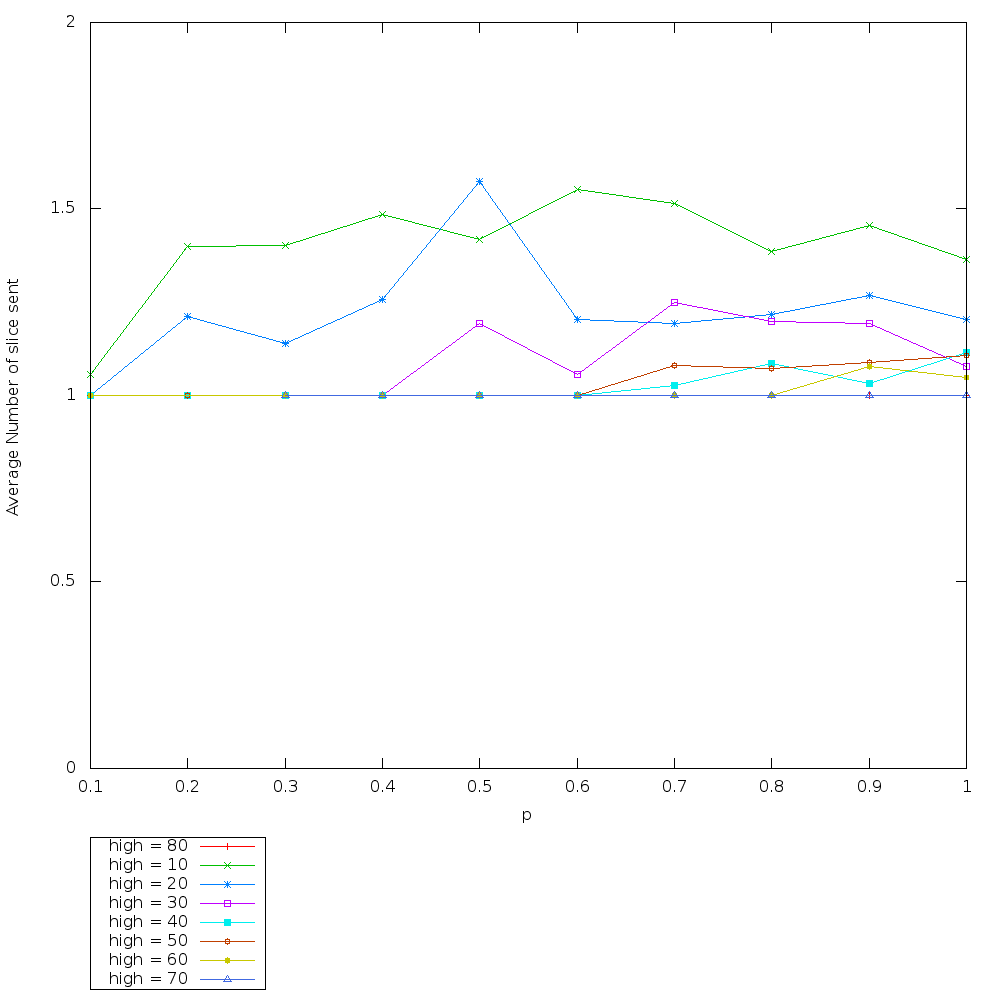
\includegraphics[height=10cm]{./image/slicesent/Nb_sent_slice.png}
  \caption{Graph of 1000 nodes with Slices of size 200}
 \end{figure}
 This graph underlines the fact that, whatever the shape of the DAG is, not a lot of slices are needed to synchronize. Therefore in this exemple the information sent by the client to synchronize fits in $20\times 320 \times 1.1 = 7040$ bits. $20$ is the number of hash functions we used, $320$ is the size of each table, and $1.1$ is the average number of slices.
 
 \paragraph{} The complexity of the explore algorithm is difficult to assert, given that it mainly depends on the shape of the tree. However we counted the number of call to the functions \texttt{pred} and \texttt{succ} of the \texttt{OcamlGraph} library as well as the number of visit to each nodes. We chose to count those calls because they are the one with the biggest complexity (according to the \texttt{OcamlGraph} documentation). The following curves shows the average values of this calls divided by the size of the difference between the DAGs depending on different values. Each DAG had $1000$ nodes labelled with $160$ bits hash.
\begin{figure}[H]
 \centering
  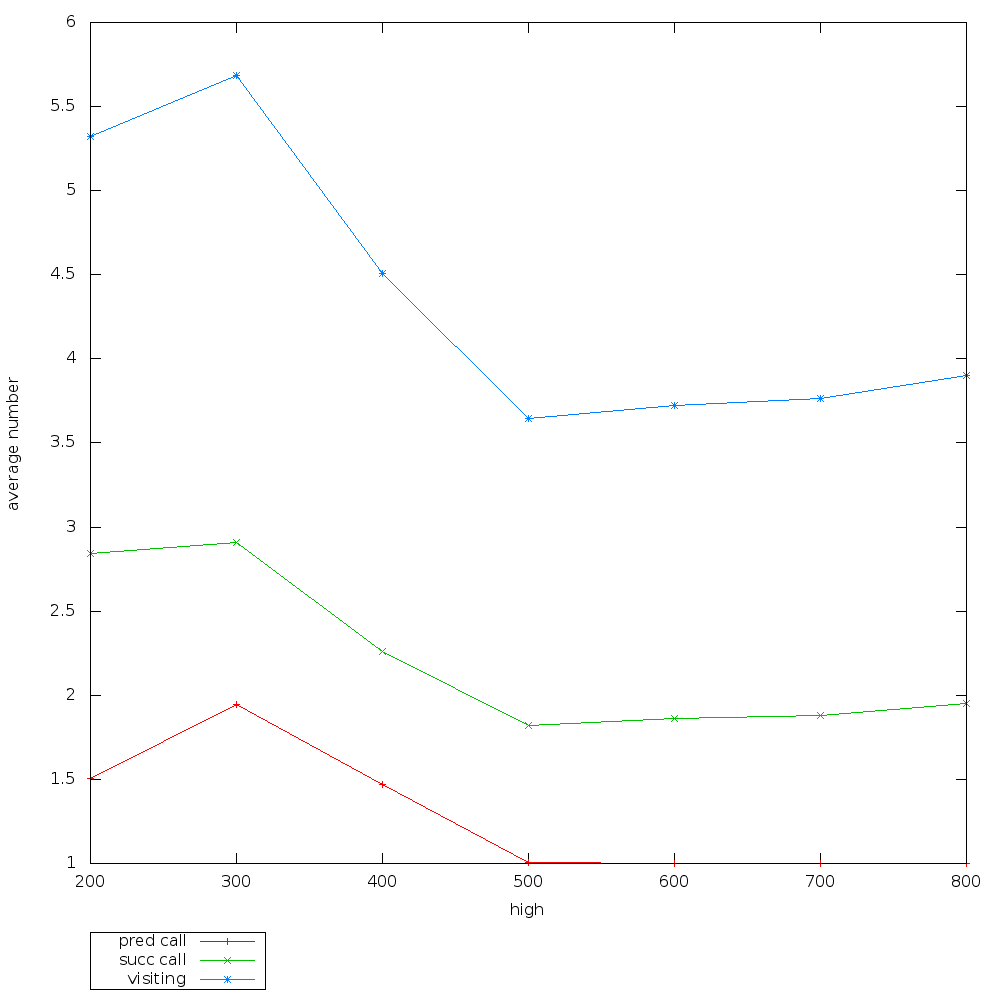
\includegraphics[height=10cm]{./image/eval/call_depending_on_high_over_size.png}
  \caption{Number of calls depending on the high of the DAG}
 \end{figure}
 \begin{figure}[H]
 \centering
  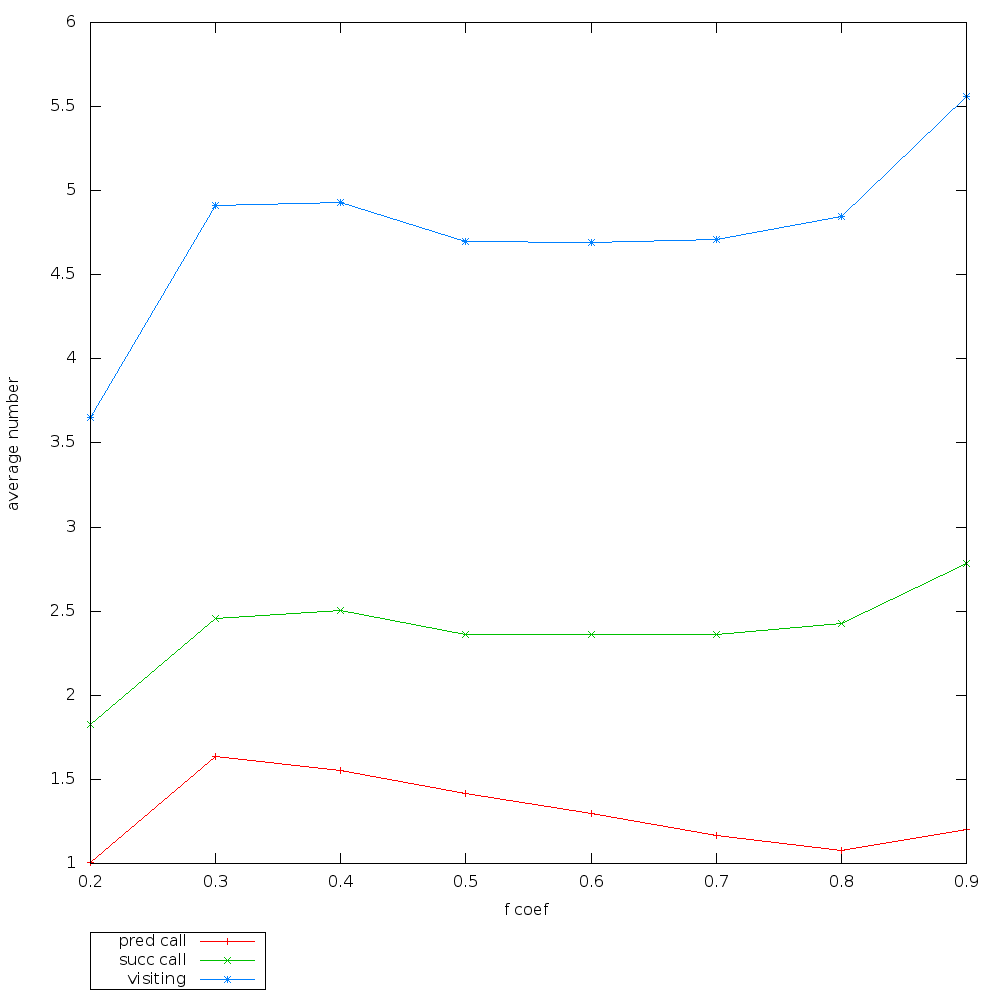
\includegraphics[height=10cm]{./image/eval/call_depending_on_f_coef.png}
  \caption{Number of calls depending on average number of predecessors}
 \end{figure}
 The two previous graphs underline that the complexity in terms of call to the \texttt{pred} and \texttt{succ} function is linear on the size of the difference between the two DAGs that are being synchronized, which is the main result we wanted. Indeed in the case where we want our algorithm to work it is important that the complexity does not increase with the size of the history but only with the size of the difference.